% Executive research summary -- Bayesian GARCH: from volatility forecasting to portfolio allocation
% Compile from this folder:  latexmk -pdf executive_summary.tex   (figures/, tables/ and references.bib are local)
% Every number is checked by scripts/verify_summary_numbers.py against the saved research tables.
\documentclass[11pt]{article}
\usepackage[letterpaper,margin=0.9in,top=0.85in,bottom=0.9in]{geometry}
\usepackage[T1]{fontenc}
\usepackage{lmodern}
\usepackage{amsmath,amssymb,booktabs,graphicx,array,xcolor,tikz,enumitem,caption,microtype,fancyhdr}
\usepackage[numbers,square,sort&compress]{natbib}
\usepackage[hidelinks]{hyperref}
\usepackage{titlesec}
\usetikzlibrary{positioning,arrows.meta,calc}
\graphicspath{{figures/}}
\hypersetup{pdfauthor={Kang Yu},pdftitle={Bayesian GARCH: Executive Research Summary}}

\definecolor{ink}{HTML}{1F1F1E}
\definecolor{muted}{HTML}{6B6A63}
\definecolor{navy}{HTML}{1D3B5C}
\definecolor{fc}{HTML}{2A78D6}
\definecolor{al}{HTML}{EB6834}
\definecolor{ex}{HTML}{1BAF7A}
\definecolor{ev}{HTML}{7A5BB5}
\definecolor{boxbg}{HTML}{EEF4FC}
\definecolor{findbg}{HTML}{FDF0EA}

\titleformat{\section}{\large\bfseries\color{navy}}{\thesection.}{0.5em}{}
\titlespacing*{\section}{0pt}{9pt}{4pt}
\titleformat{\subsection}{\normalsize\bfseries\color{navy}}{}{0em}{}
\titlespacing*{\subsection}{0pt}{6pt}{2pt}
\setlist{itemsep=1pt,topsep=2pt,leftmargin=1.3em}
\captionsetup{font=small,labelfont={bf,color=navy},skip=4pt}
\setlength{\parskip}{3pt}\setlength{\parindent}{0pt}
\pagestyle{fancy}\fancyhf{}
\renewcommand{\headrulewidth}{0.4pt}
\fancyhead[L]{\small\color{muted}Bayesian GARCH \textbar{} Executive research summary}
\fancyhead[R]{\small\color{muted}Kang Yu \textbar{} November 2026}
\fancyfoot[C]{\small\thepage}

\newcommand{\E}{\mathbb{E}}
\newcommand{\Var}{\operatorname{Var}}
\newcommand{\logit}{\operatorname{logit}}
\newcommand{\pbox}[1]{\par\smallskip\noindent\colorbox{boxbg}{\parbox{\dimexpr\textwidth-2\fboxsep}{#1}}\par\smallskip}
\newcommand{\finding}[2]{\par\smallskip\noindent\colorbox{findbg}{\parbox{\dimexpr\textwidth-2\fboxsep}{\textbf{\color{al}#1.} #2}}\par\smallskip}

\begin{document}
\thispagestyle{fancy}
\begin{center}
{\LARGE\bfseries\color{navy} Bayesian GARCH: From Volatility Forecasting\\[2pt] to Portfolio Allocation}\\[6pt]
{\large Executive research summary}\\[4pt]
Kang Yu \;\textperiodcentered\; Erd\H{o}s Institute, Quantitative Methods in Finance \;\textperiodcentered\; November 2026
\end{center}

\pbox{\textbf{In brief.} Four ETFs are forecast strictly out of sample with Gaussian GARCH(1,1), estimated by maximum
likelihood (MLE) and by Bayesian MCMC, and with Student-$t$ GARCH (MLE). Integrating over posterior parameter
uncertainty gives \emph{no statistically reliable} improvement in variance forecasts (H1), a \emph{small but reliable}
improvement in predictive densities (H2), and \emph{no reliable} investment benefit once risky exposure is controlled
(H3). The two results that define the project: \textbf{(1)} Student-$t$ innovations improve density forecasts about five
to six times as much as Bayesian integration in the primary period; \textbf{(2)} the conservative Bayesian portfolio's
smaller drawdowns disappear against an \textbf{exposure-matched MLE control}.}

% =====================================================================================================
\section{Research question and motivation}
\textbf{Question.} \emph{Does accounting for Bayesian parameter uncertainty improve conditional variance forecasts,
predictive return distributions, and volatility-targeted investment performance?}

Daily returns are nearly unpredictable, but their \emph{size} is not: large moves cluster (for SPY, the lag-1
autocorrelation of squared returns is 0.42). GARCH \cite{engle1982,bollerslev1986} models this clustering with a few parameters estimated from a few
noisy years, yet the standard forecast plugs in the point estimate as if it were exact. Returns are also heavy-tailed,
so the shape of the predictive distribution matters, not just its variance; and a statistically better forecast need
not produce a better investment decision. This motivates three hypotheses:

\begin{description}[leftmargin=2.3em,style=sameline]
\item[H1] Bayesian parameter integration improves one-day-ahead \textbf{conditional variance} forecasts relative to Gaussian GARCH MLE.
\item[H2] It improves the full \textbf{predictive distribution} of daily returns.
\item[H3] Using posterior uncertainty in volatility targeting improves \textbf{investment outcomes beyond merely reducing risky exposure}.
\end{description}

% =====================================================================================================
\section{Statistical methodology}
\textbf{Gaussian GARCH(1,1).} For the daily log return $r_t$ with information $\mathcal F_{t-1}$,
\begin{equation}
r_t=\sqrt{h_t}\,z_t,\quad z_t\overset{iid}{\sim}N(0,1),\qquad h_t=\omega+\alpha r_{t-1}^2+\beta h_{t-1},
\end{equation}
where $h_t=\Var(r_t\mid\mathcal F_{t-1})$ is the conditional variance, $\omega>0$, $\alpha,\beta\ge0$, and the
\emph{persistence} $\alpha+\beta<1$ sets how slowly shocks decay toward the long-run variance $\omega/(1-\alpha-\beta)$.
MLE maximises $\ell(\theta)=-\frac12\sum_t[\log2\pi+\log h_t(\theta)+r_t^2/h_t(\theta)]$ in unconstrained coordinates
(log long-run variance and two logits), giving one estimate $\hat\theta$.

\textbf{Bayesian Gaussian GARCH.} The posterior $p(\theta\mid D)\propto p(D\mid\theta)\,p(\theta)$ \cite{ardia2008} uses weakly
informative normal priors on the same coordinates and is sampled by adaptive random-walk Metropolis \cite{roberts1997,haario2001} (4 chains, 2{,}500
warm-up and 4{,}000 retained iterations each; a fit passes only if $\hat R<1.01$ and bulk and tail ESS $\ge400$ \cite{vehtari2021}). Each
of $M=300$ posterior draws, sampled at random from the retained draws, runs its own recursion and yields a forecast
$h_t^{(m)}$. Three summaries are used, one per hypothesis:
\begin{equation}
\text{H1: }\bar h_t=\frac1M\sum_m h_t^{(m)},\qquad
\text{H2: }p_{\text{Bayes}}(r)=\frac1M\sum_m N\bigl(r;0,h_t^{(m)}\bigr),\qquad
\text{H3: }q_{0.9,t}=Q_{0.9}\{h_t^{(m)}\}.
\end{equation}
The predictive density averages the component \emph{densities}; its log score is computed with log-sum-exp.

\textbf{Student-$t$ GARCH (MLE)} \cite{bollerslev1987}. The same variance recursion with standardised Student-$t$ innovations,
$z_t=\sqrt{(\nu-2)/\nu}\,T_\nu$ ($\nu>2$, unit variance). The four parameters $(\omega,\alpha,\beta,\nu)$ are estimated
jointly by maximum likelihood at every refit; smaller $\nu$ means heavier tails (excess kurtosis $6/(\nu-4)$ for
$\nu>4$). The fitted $\nu$ has a median of 7.2 over the 320 refits.

\pbox{\textbf{Two different routes to heavier predictive tails.} \emph{Bayesian Gaussian GARCH} mixes Gaussians whose
variances differ across parameter draws; how much tail this adds depends on how dispersed the forecasts
$h_t^{(m)}$ are. \emph{Student-$t$ GARCH} builds heavy-tailed innovations into the conditional model itself. A
classical Laplace approximation (draws from $N(\hat\theta,\hat{\mathcal I}^{-1})$) and EWMA \cite{riskmetrics1996} serve as secondary comparators.}

% =====================================================================================================
\section{Data and rolling experimental design}
Daily split- and dividend-adjusted closes of SPY and QQQ (US equities), TLT (long Treasuries) and GLD (gold) from
January 2013 to 4 November 2026 are converted to log returns; cash earns the effective federal funds rate. No model is
ever fitted on the whole history. At each refit date, every model is estimated on the latest $W=500$ or $1{,}000$
returns only; the parameters are then frozen for the next \textbf{63 trading days}, while every model's variance is
updated \textbf{daily} with newly observed returns to produce one-step-ahead forecasts. Each forecast is scored only
after its return is observed. Four ETFs $\times$ two windows $\times$ two periods give 320 refits (Figure~\ref{fig:design}).

\begin{figure}[h]\centering
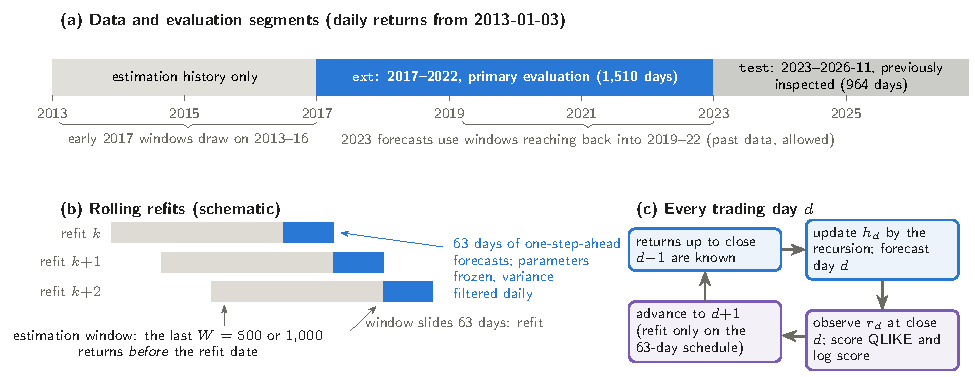
\includegraphics[width=\textwidth]{rolling_design.pdf}
\caption{Rolling out-of-sample design: (a) evaluation segments; (b) refits on the latest window, then 63 days of
forecasts with frozen parameters; (c) the daily forecast--observe--score loop.}\label{fig:design}
\end{figure}

\textbf{Evaluation periods.} 2017--2022 (\texttt{ext}, 1{,}510 days per ETF) is the \emph{primary} evaluation: models,
metrics and decision rules were frozen before any of its results were examined, so it is independent of
research-development \emph{inspection}; its returns are of course not statistically independent of other years.
2023--2026 (\texttt{test}, 964 days) had been inspected during development and is reported as a reproduction. Both are
chronological out-of-sample periods, and earlier returns legitimately enter later estimation windows.

% =====================================================================================================
\section{H1 --- conditional variance forecasting}
\textbf{Question.} Does the posterior-integrated forecast $\bar h_t$ beat the MLE forecast $h_t(\hat\theta)$?

\textbf{Metric.} The true conditional variance is latent; the squared return is an unbiased but very noisy proxy,
$\E[r_t^2\mid\mathcal F_{t-1}]=h_t$. Forecasts are scored with
\begin{equation}
\text{QLIKE}_t(\hat h)=\log\hat h_t+r_t^2/\hat h_t\qquad\text{(lower is better)},
\end{equation}
which equals twice the Gaussian negative log-likelihood minus $\log2\pi$. Its conditional expectation,
$\log\hat h+h_t/\hat h$, is uniquely minimised at $\hat h=h_t$, whenever the conditional second moment exists and
whatever the shape of the return distribution \cite{patton2011}. The proxy noise therefore does not bias the ranking \emph{in
expectation}; it does make single days uninformative, so average differences are tested. Daily differences are
pooled across the four ETFs and tested with Diebold--Mariano statistics \cite{diebold1995} using Newey--West standard errors \cite{neweywest1987}.

\begin{table}[h]\centering\small
\resizebox{\textwidth}{!}{\begin{tabular}{lcc@{\qquad}cc}
\toprule
Bayes integrated $-$ MLE, mean daily QLIKE difference & \multicolumn{2}{c}{2017--22 (primary)} & \multicolumn{2}{c}{2023--26 (inspected)}\\
 & 500-day & 1{,}000-day & 500-day & 1{,}000-day\\
\midrule
difference & $-0.00534$ & $-0.00558$ & $-0.00331$ & $-0.00085$\\
95\% Newey--West interval & $[-0.0118,\,0.0011]$ & $[-0.0117,\,0.0006]$ & $[-0.0084,\,0.0018]$ & $[-0.0032,\,0.0015]$\\
$p$-value & 0.105 & 0.076 & 0.206 & 0.484\\
\bottomrule
\end{tabular}}
\caption{H1. Negative values favour the Bayesian forecast. Average QLIKE levels are about $-8.3$.}\label{tab:h1}
\end{table}

\textbf{H1 conclusion.} The differences numerically favour the Bayesian forecast but are not significant at the 5\%
level in any cell: \emph{no statistically reliable improvement was established}. The intervals include both zero and
small gains, so this is not evidence that the forecasts are equivalent.

% =====================================================================================================
\section{H2 --- predictive return distributions}
\textbf{Question.} Does integrating parameter uncertainty improve the \emph{whole} predictive distribution? Two
forecasts with nearly the same variance can assign very different probabilities to a crash, which QLIKE cannot see.

\textbf{Metric.} The log predictive score $S_t=\log p(r_t^{\text{obs}}\mid D_{t-1})$ (higher is better) evaluates the
density, stated before the return is observed, at the realised return. It is strictly proper \cite{gneiting2007}: in expectation it is
maximised only by the true predictive distribution. For a single Gaussian it ranks forecasts exactly like QLIKE; for a
mixture or a Student-$t$ density it also rewards the \emph{shape}, in particular the tail mass. Three densities are
compared: the Gaussian MLE plug-in, the Bayesian predictive mixture, and Student-$t$ GARCH (MLE).

\begin{table}[h]\centering\small
\resizebox{\textwidth}{!}{\begin{tabular}{lcccc}
\toprule
Mean daily log-score gain over Gaussian MLE (nats) & \multicolumn{2}{c}{2017--22 (primary)} & \multicolumn{2}{c}{2023--26 (inspected)}\\
 & 500-day & 1{,}000-day & 500-day & 1{,}000-day\\
\midrule
Bayesian Gaussian mixture & $+0.00518$ \small($p=0.012$) & $+0.00469$ \small($p=0.024$) & $+0.00519$ & $+0.00226$\\
Student-$t$ GARCH (MLE) & $+0.02822$ \small($p<0.001$) & $+0.02865$ \small($p<0.001$) & $+0.01887$ & $+0.01699$\\
Student-$t$ $-$ Bayesian mixture & $+0.02303$ \small($p<0.001$) & $+0.02396$ \small($p<0.001$) & $+0.01369$ & $+0.01473$\\
\midrule
Student-$t$ gain $\div$ Bayesian gain & 5.44 & 6.11 & 3.64 & 7.52\\
Laplace gain $\div$ Bayesian gain & 0.89 & 0.43 & 0.82 & 0.69\\
\bottomrule
\end{tabular}}
\caption{H2. Pooled four-ETF contrasts; $p$-values from Newey--West Diebold--Mariano tests. In 2023--26 all
Bayesian gains have $p\le0.024$ and all Student-$t$ comparisons $p\le0.011$.}\label{tab:h2}
\end{table}

The Bayesian mixture beats the MLE density in every cell, but only by 0.002--0.005 nats per day, and a classical
Laplace approximation recovers 43--89\% of that gain without MCMC. Student-$t$ GARCH gains about \textbf{5.4 and 6.1
times as much} in the primary period; across all four cells the ratio ranges from 3.6 to 7.5, so no single multiplier
applies everywhere. Student-$t$ also beats the Bayesian mixture directly in every cell.

\begin{figure}[h]\centering
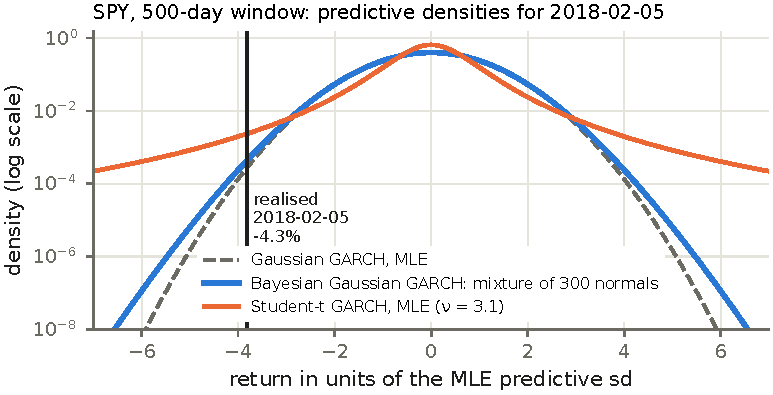
\includegraphics[width=.74\textwidth]{predictive_densities.pdf}
\caption{Predictive densities for SPY (500-day window) on 5 February 2018, from the saved model estimates, on a log
scale. The date was \emph{selected to illustrate a tail event} ($-4.3\%$, 3.8 MLE standard deviations) and is not
typical. The three variances are within 5\%, yet the realised return's density is 8.6 times higher under
Student-$t$ ($\hat\nu=3.1$ on this refit) than under the Gaussian MLE.}\label{fig:dens}
\end{figure}

\textbf{Why Student-$t$ does so much better.} Gaussian GARCH already captures volatility clustering, and time-varying
variance already makes \emph{unconditional} returns heavy-tailed; the question is whether the \emph{conditional} tails
are right. Bayesian integration adds one more Gaussian scale mixture. If $r=\sqrt{H}\,z$ with $z\sim N(0,1)$
independent of the mixing variance $H$ (here $H$ is uniform over the posterior forecasts $h_t^{(m)}$),
\begin{equation}
\kappa_{\text{excess}}=\frac{\E r^4}{(\E r^2)^2}-3=3\,\frac{\Var(H)}{\E[H]^2}=3\,\mathrm{CV}(H)^2 .
\end{equation}
The posterior forecast dispersion is small: CV of 7--12\% on average, and the day-average of $3\,\mathrm{CV}^2$ is
only 0.015--0.046. Returns standardised by the Bayesian forecast show excess kurtosis of 0.4--2.9, so parameter
uncertainty explains only a few per cent of the tail heaviness. Student-$t$ innovations supply it directly
(with $\nu\approx7$, $6/(\nu-4)\approx2$). Tail calibration agrees: 1\% value-at-risk is breached on 2.2\% (MLE) and
2.1\% (Bayesian mixture) of days in 2017--22, against 1.5\% for Student-$t$.

\finding{Finding 1 --- H2}{Bayesian parameter integration modestly but significantly improves density forecasts;
modelling heavy-tailed innovations with Student-$t$ GARCH produces a substantially larger gain. Within the tested
Gaussian model, innovation misspecification matters more than parameter uncertainty. This does not show that
parameter uncertainty is unimportant in general; a Bayesian Student-$t$ GARCH was not tested.}

% =====================================================================================================
\section{H3 --- from forecasts to portfolios}
\textbf{Question.} Do better probabilistic forecasts produce better investment decisions? Each strategy holds a
fraction of wealth in one ETF and the rest in cash, targeting 10\% annual volatility without leverage
(volatility targeting \cite{moreira2017}):
\begin{equation}
w_d=\min\Bigl(1,\ \frac{k_d\cdot0.10}{\sqrt{252\,h_d}}\Bigr),\qquad k_d=1\text{ except for the control below}.
\end{equation}
The strategies differ only in the variance used: the MLE forecast $\hat h_d$, the posterior mean $\bar h_d$, or the
posterior 90th percentile $q_{0.9,d}$ (``upper-90''), a deliberately conservative, preselected policy rather than an
optimised threshold. Higher forecast variance means a smaller ETF weight.

\begin{figure}[h]\centering
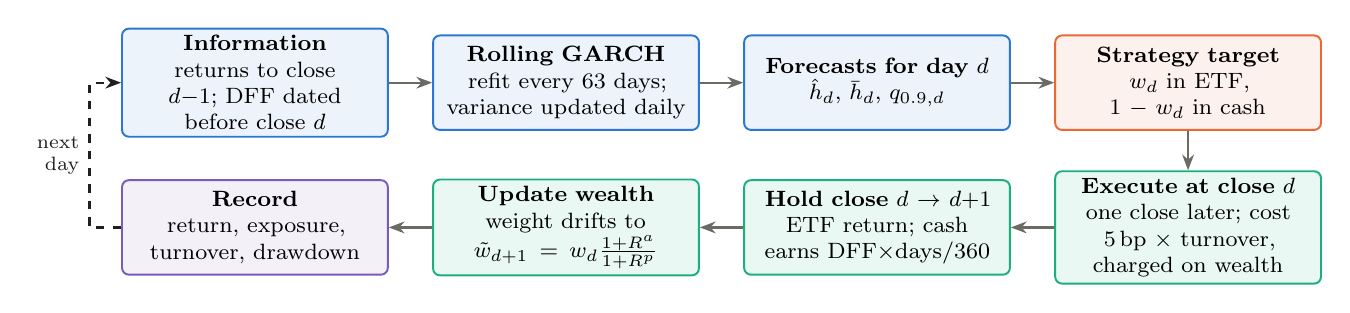
\begin{tikzpicture}[
  bx/.style={draw=#1, fill=#1!9, line width=0.7pt, rounded corners=2.5pt, align=center, text width=3.2cm,
             minimum height=1.2cm, font=\footnotesize, inner sep=2.5pt},
  ar/.style={-{Stealth[length=2mm]}, line width=0.8pt, draw=muted}, node distance=5mm and 5.5mm]
\node[bx=fc] (a) {\textbf{Information}\\returns to close $d{-}1$; DFF dated before close $d$};
\node[bx=fc, right=of a] (b) {\textbf{Rolling GARCH}\\refit every 63 days; variance updated daily};
\node[bx=fc, right=of b] (c) {\textbf{Forecasts for day $d$}\\$\hat h_d$, $\bar h_d$, $q_{0.9,d}$};
\node[bx=al, right=of c] (d) {\textbf{Strategy target}\\$w_d$ in ETF, $1-w_d$ in cash};
\node[bx=ex, below=of d] (e) {\textbf{Execute at close $d$}\\one close later; cost 5\,bp $\times$ turnover, charged on wealth};
\node[bx=ex, left=of e] (f) {\textbf{Hold close $d\to d{+}1$}\\ETF return; cash earns DFF$\times$days/360};
\node[bx=ex, left=of f] (g) {\textbf{Update wealth}\\weight drifts to $\tilde w_{d+1}=w_d\frac{1+R^a}{1+R^p}$};
\node[bx=ev, left=of g] (h) {\textbf{Record}\\return, exposure, turnover, drawdown};
\draw[ar] (a)--(b); \draw[ar] (b)--(c); \draw[ar] (c)--(d); \draw[ar] (d)--(e); \draw[ar] (e)--(f); \draw[ar] (f)--(g); \draw[ar] (g)--(h);
\draw[ar, dashed, draw=ink] (h.west) -- ++(-4mm,0) |- node[pos=.25, left, font=\scriptsize, align=right, text=ink]{next\\day} (a.west);
\end{tikzpicture}
\caption{Portfolio simulation as implemented, one trading day. Blue: forecasting; orange: allocation; green: execution
and accounting; purple: evaluation. The portfolio is rebalanced to target every day (executed weight $=$ target);
costs reduce wealth, returns make the weight drift, and parameters change only at the 63-day refits.}\label{fig:flow}
\end{figure}

\textbf{Accounting.} With ETF simple return $R^a_{d+1}$ and cash return $R^f_{d+1}$, wealth evolves as
$W_{d+1}=W_d(1-c_d)\bigl(1+w_dR^a_{d+1}+(1-w_d)R^f_{d+1}\bigr)$, starting from $W_0=1$ in cash. No forecast uses a
return that has not been observed, and the trade is executed one close after the information that produced it.

% =====================================================================================================
\section{H3 --- evaluation in two stages}
\textbf{Metrics.} The Sharpe ratio is the mean daily return in excess of cash divided by the standard deviation of
that excess return, times $\sqrt{252}$; the maximum drawdown is the worst peak-to-trough fall in wealth. Realised
volatility and average ETF exposure complete the picture. Two aggregations are used and must not be confused:
\emph{means over the eight single-ETF asset/window configurations} (Tables~\ref{tab:stage1}--\ref{tab:stage2}) and the
\emph{equal-weight four-ETF sleeve} (Table~\ref{tab:sleeve}). Uncertainty comes from paired circular block-bootstrap
intervals \cite{politis1992} (20-day blocks, 2{,}000 replications).

\subsection{Stage 1: Bayesian upper-90 versus standard MLE}
\begin{table}[h]\centering\small
\resizebox{.92\textwidth}{!}{\begin{tabular}{lrrrrr}\toprule
2017--22, mean of 8 single-ETF configurations & Exposure & Return & Volatility & Sharpe & Max DD\\\midrule
Standard MLE & 73.1\% & 6.25\% & 10.37\% & 0.518 & $-19.55\%$ \\
Bayesian upper-90 & 69.6\% & 6.06\% & 9.81\% & 0.520 & $-18.74\%$ \\
\midrule
Difference (upper-90 $-$ MLE) & $-3.6$ pp & $-0.19$ pp & $-0.55$ pp & $+0.002$ & $+0.82$ pp \\
Configurations whose 95\% CI excludes 0 & & & & 0 of 8 & 8 of 8 \\
\bottomrule\end{tabular}
}
\caption{Stage 1, 2017--22: means over the 8 single-ETF configurations, 5 bp costs. The last row counts configurations
whose paired 95\% interval for the difference excludes zero.}\label{tab:stage1}
\end{table}

\textbf{Observation.} Upper-90 has lower volatility (9.81\% versus 10.37\%) and a shallower maximum drawdown, by 0.82
points on average; its drawdown is smaller in all 8 configurations and every drawdown interval excludes zero. But it
also holds 3.6 points less ETF, and its Sharpe ratio is nearly unchanged: no configuration interval excludes zero
(sleeve: $+0.011$ $[-0.021,\,0.042]$ and $+0.000$ $[-0.025,\,0.026]$).
\textbf{Interpretation.} Upper-90 takes less risk at almost the same risk-adjusted return, the pattern a lower
volatility target would also produce. The table cannot say why its drawdown is lower.

\pbox{\textbf{Question raised by Stage 1.} Does Bayesian uncertainty improve allocation \emph{timing}, or is the lower
drawdown simply a consequence of \emph{holding less risk}?}

\subsection{Stage 2: the exposure-matched MLE control}
\textbf{Objective.} Hold upper-90's average risk with \emph{no} posterior information: if upper-90 only holds less risk,
the two should tie; if the posterior improves timing, upper-90 should still win. The control keeps the MLE variance
forecast unchanged and scales only the volatility target:
\begin{equation}
\begin{gathered}
w^{\text{ctrl}}_d=\min\Bigl(1,\frac{k_d\cdot0.10}{\sqrt{252\,\hat h_d}}\Bigr),\\
k_d=\frac{1}{d-\max(0,d-252)}\sum_{s=\max(0,d-252)}^{d-1}\sqrt{\frac{\hat h_s}{q_{0.9,s}}}\quad(d\ge1),\qquad k_0=\sqrt{\hat h_0/q_{0.9,0}}.
\end{gathered}
\end{equation}
$k_d$ is the trailing mean, over up to 252 earlier forecast rows, of the ratio of MLE to upper-90 volatility forecasts
(the ratio of their uncapped weights); the first row uses its own ratio, known at decision time. It moves the
\emph{effective volatility target} $0.10\,k_d$, not the GARCH parameters or the variance forecast. No realised return
enters $k_d$ directly (only earlier forecasts, themselves built from past returns), no future information is used,
and the posterior never enters the MLE forecast. It matches upper-90's average \emph{haircut}, so exposure is
matched only approximately (mean gap $+0.1$ pp, range $-0.06$ to $+0.41$ pp, because weights are capped at one), and
equal average exposure does not imply equal daily risk. Execution, costs and cash accounting are identical.

\begin{table}[h]\centering\small
\resizebox{.92\textwidth}{!}{\begin{tabular}{lrrrrr}\toprule
2017--22, mean of 8 single-ETF configurations & Exposure & Return & Volatility & Sharpe & Max DD\\\midrule
Exposure-matched MLE & 69.4\% & 6.01\% & 9.85\% & 0.516 & $-18.66\%$ \\
Bayesian upper-90 & 69.6\% & 6.06\% & 9.81\% & 0.520 & $-18.74\%$ \\
\midrule
Difference (upper-90 $-$ matched MLE) & $+0.1$ pp & $+0.04$ pp & $-0.03$ pp & $+0.003$ & $-0.07$ pp \\
Configurations whose 95\% CI excludes 0 & & & & 0 of 8 & 0 of 8 \\
\bottomrule\end{tabular}
}
\caption{Stage 2, 2017--22: the same metrics for upper-90 and the exposure-matched control.}\label{tab:stage2}
\end{table}

\textbf{Observation.} Once average exposure is matched, volatility (9.81\% versus 9.85\%), maximum drawdown
($-18.74\%$ versus $-18.66\%$) and Sharpe ratio (0.520 versus 0.516) are very similar; upper-90's drawdown is smaller
in only 2 of 8 configurations, and no configuration interval excludes zero for either metric. At the sleeve level
(Table~\ref{tab:sleeve}) the drawdown advantage over MLE is clear, but against the control it vanishes, and every
Sharpe-difference interval contains zero, as do all 12 sleeve intervals across both periods and the Laplace comparison.

\begin{table}[h]\centering\small
\resizebox{\textwidth}{!}{\begin{tabular}{llrr}
\toprule
2017--22, equal-weight four-ETF sleeve & & $\Delta$Sharpe [95\% CI] & $\Delta$Max DD, pp [95\% CI]\\
\midrule
Stage 1: upper-90 $-$ MLE & 500-day & $+0.011$ $[-0.021,\,0.042]$ & $+0.76$ $[0.22,\,1.21]$\\
 & 1{,}000-day & $+0.000$ $[-0.025,\,0.026]$ & $+0.55$ $[0.11,\,1.01]$\\
Stage 2: upper-90 $-$ exposure-matched MLE & 500-day & $+0.009$ $[-0.016,\,0.036]$ & $-0.01$ $[-0.22,\,0.43]$\\
 & 1{,}000-day & $+0.005$ $[-0.016,\,0.027]$ & $-0.03$ $[-0.20,\,0.45]$\\
\bottomrule
\end{tabular}}
\caption{Paired differences with circular block-bootstrap intervals. Positive $\Delta$Max DD means a shallower drawdown
for upper-90.}\label{tab:sleeve}
\end{table}

\begin{figure}[h]\centering
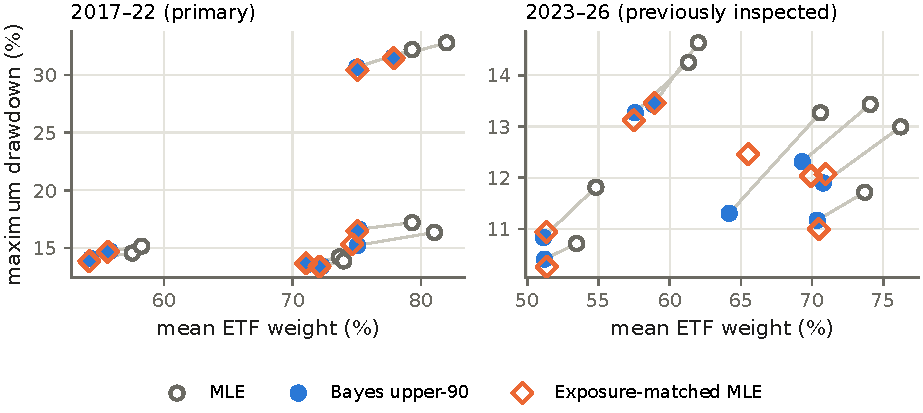
\includegraphics[width=.8\textwidth]{exposure_control.pdf}
\caption{Mean ETF weight versus maximum drawdown for each asset/window configuration. Grey lines join MLE to upper-90
(Stage 1); the exposure-matched control (diamonds, Stage 2) lands on top of upper-90 in both periods.}\label{fig:exp}
\end{figure}

\textbf{Interpretation.} The Stage 1 drawdown advantage is reproduced by a strategy that holds the same average risk
without any posterior information. The Sharpe point estimates are small and their intervals a few hundredths wide, so
no statistically reliable incremental benefit is established, and the rounded point estimates should not be read as a
gain or a loss. The upper-90 weights are very close to a constant haircut of the MLE weights, which is what a lower
volatility target would do.

\finding{Finding 2 --- H3}{The observed drawdown reduction is largely consistent with lower average risky exposure rather
than demonstrably superior risk timing from Bayesian parameter uncertainty; the tested strategy shows no reliable
advantage over an exposure-matched MLE control. This limits what the tested rules show; it is not proof that
Bayesian uncertainty can have no economic value.}

% =====================================================================================================
\section{Limitations and future research}
\begin{itemize}
\item \textbf{Model scope.} Only Gaussian GARCH(1,1) receives a Bayesian treatment; equity residuals are also
negatively skewed, which no symmetric model captures.
\item \textbf{Estimation.} Finite 500/1{,}000-day windows, quarterly refits, and the MLE persistence bound, which binds in
30 of 320 refits. MCMC output is random: 4 of 320 fits miss the strict convergence rule marginally, and Bayesian
results reproduce to Monte Carlo precision, not bit-for-bit, across platforms.
\item \textbf{Inference.} Returns and score differences are serially dependent (handled with HAC and block-bootstrap
methods), and four ETFs over six plus four years cannot resolve Sharpe differences below about 0.05.
\item \textbf{Backtest.} Close-to-close execution one close after the signal, proportional 5 bp costs and the federal
funds rate as cash are approximations shared by all strategies; average exposure matching is not full risk equalisation.
\end{itemize}
\textbf{Future work (not tested):} Bayesian Student-$t$ and skewed-$t$ GARCH; hierarchical priors across assets; and
uncertainty-aware allocation objectives such as utility maximisation or expected-shortfall targeting, always evaluated
against matched controls.

% =====================================================================================================
\section{Summary}
\pbox{\begin{tabular}{@{}l@{\;\;}p{0.8\textwidth}@{}}
\textbf{H1} & \textbf{Conditional variance.} Small numerical QLIKE improvements ($-0.0053$ and $-0.0056$ in 2017--22,
$p=0.105$ and $0.076$); no statistically reliable improvement at 5\%.\\[2pt]
\textbf{H2} & \textbf{Predictive distribution.} A small, reliable Bayesian gain (0.002--0.005 nats/day); Student-$t$
GARCH (MLE) gains 5.4--6.1 times as much in 2017--22.\\[2pt]
\textbf{H3} & \textbf{Investing.} Conservative Bayesian targeting lowers exposure and drawdowns, but not reliably beyond
an exposure-matched MLE policy.
\end{tabular}}
\textbf{Finding 1 --- statistical forecasting.} Modelling heavy-tailed innovations had a substantially larger effect on
predictive-density accuracy than Bayesian integration under the Gaussian GARCH specification.

\textbf{Finding 2 --- investment evaluation.} Reduced drawdowns from conservative Bayesian allocation were largely
explained by lower average risky exposure; the tested strategy did not establish a reliable advantage over an
exposure-matched MLE control.

\textbf{Research lesson.} \emph{Better probabilistic forecasts do not automatically produce better investment
decisions. Understanding model misspecification and using appropriate experimental controls are essential for
evaluating economic value.}

\medskip
{\footnotesize\raggedright\color{muted}\textbf{Evidence and reproducibility.} Every number in this summary is checked against the
saved research tables by \texttt{scripts/verify\_summary\_numbers.py}. The full report (\texttt{research\_report.pdf}) gives derivations,
all tables and appendices; \texttt{quick\_walkthrough.ipynb} and \texttt{walkthrough.ipynb} rerun representative MLE,
MCMC and Student-$t$ fits and recompute every metric from the saved daily forecasts (45 and 130 automated checks; 54
unit tests). A full rebuild of all 320 refits from market data reproduced every table column exactly on the
development machine; on other platforms Bayesian quantities agree to Monte Carlo precision. Data: Yahoo Finance
adjusted closes (not redistributed) and FRED DFF.
The analysis code, experiments and text were produced with substantial assistance from an AI system (Claude, by
Anthropic) under the author's direction; all quantitative statements were checked programmatically.\par}
{\footnotesize\setlength{\bibsep}{1.5pt}
\bibliographystyle{unsrtnat}
\bibliography{references}}
\end{document}
